\paragraph{Single crystals}
Single crystals show a nicely ordered, clean surface - two properties important for reliable and reproducible experiments. We have chosen both silver and copper as bulk crystalline substrates. Both form fcc lattices and their surface termination can be chosen by precise cutting along a symmetry plane of choice. For the course of this thesis, experiments are conducted mainly on (111) and (100) terminated surfaces.\footnote{See \cite{riemann_ionic_2002} and appendix \fullref{appendix:crystal-facets} for another examples of vicinal metal surfaces (531), (532), (221), (311), (211).} Commercially available, single crystals guarantee a high precision in facet orientation and purity (99.999 \%) \cite{mateck}. Remaining contaminations in copper (Ag: \SI{0.8}{ppm}, Pb: \SI{0.3}{ppm}, Bi: \SI{0.8}{ppm}) and silver (Cu: \SI{2}{ppm}, Fe: \SI{2}{ppm}, Au: \SI{0.8}{ppm}, Ni: \SI{0.8}{ppm}) are removed by repeated sputter\footnote{$U_{accel}=\SIrange{800}{1000}{\volt}$, $T_{sample}\approx \SI{300}{\kelvin}$} and anneal cycles\footnote{Cu: $T_{sample}=\SI{750}{\celsius}$, Ag: $T_{sample}=\SI{450}{\celsius}$, Au\/Mica: $T_{sample}= \underline{\textbf{get value: 450?}}$} in UHV. Typical cool down temperatures $\leq 5 \frac{K}{s}$ result in a smooth, atomically flat surface with large terrace size. 

The lattice constants at room temperatures for \underline{\textbf{cite!}} Cu(\SI{3,61}{\angstrom}), Ag(\SI{4,09}{\angstrom}) and Au(\SI{4,07}{\angstrom}) are related to the environment temperatures by their expansion coefficients.
Coefficients of \SI{16,5e-6}{\per \kelvin}(Cu), \SI{18,9e-6}{\per \kelvin}(Ag) and \SI{14,2e-6}{\per \kelvin}(Au) make the substrate lattice shrink by $\approx \SI{0,5}{\percent}$ when it is cooled down from RT to low temperature measurement conditions in STM/AFM (\SIrange{5}{7}{\kelvin}). While rather negligible for bulk materials that are not heated and cooled over larger temperature ranges, the small change in substrate lattice size may introduce strain in grown ad layers since these are grown via CVD typically at elevated temperatures and may have partially negative thermal expansion coefficients\cite{farwick_zum_hagen_structure_2016}.

%\begin{table}
%\centering \index{Crystal:lattice constants}
%\caption{Inter atomic distances for Cu and Ag with respect to different surface termination. $a$ denotes the lattice constant and $\beta= \SI{60}{\deg}$ the angle within the (111) unit cell}
%  \begin{tabular}{ccccc}
%& Lattice constant a [\SI{}{\angstrom}] & Nearest neighbors [\SI{}{\angstrom}] & diagonal [\SI{}{\angstrom}]\\ \hline 
%\multicolumn{2}{c}{fcc(100)} & $\frac{\sqrt{2}a}{2}$ & a \\
%  Cu	 	& 3.61	& 2.55 | 2.55 & 3.61  \\
%  Ag		& 4.09	& 2.89 | 2.89 & 4.09 \\ \hline 
%\multicolumn{2}{c}{fcc(111)} & $\frac{\sqrt{2}a}{2} \ <110>$ & $\sqrt{2}a\sin(\frac{\beta}{2})$ | $\sqrt{2}a\cos(\frac{\beta}{2})$\\
%Cu 		& 3.61	& 2.55 | 2.55	& 2.55 | 4.42 \\
%Ag		& 4.09	& 2.89 | 2.89	& 2.89 | 5.01 \\ \hline
%%
%%\multicolumn{2}{c}{fcc(110)} & $\frac{\sqrt{2}a}{2}$ | a & $\sqrt{\frac{3}{2}}a$\\
%%  Cu	 	& 3.61	& 2.55 | 3.61	& 4.42 \\
%%  Ag		& 4.09	& 2.89 | 4.09	& 5.00 \\ \hline 
% \end{tabular}
%\end{table}

\begin{figure}\centering
	\subfigure[(111)]{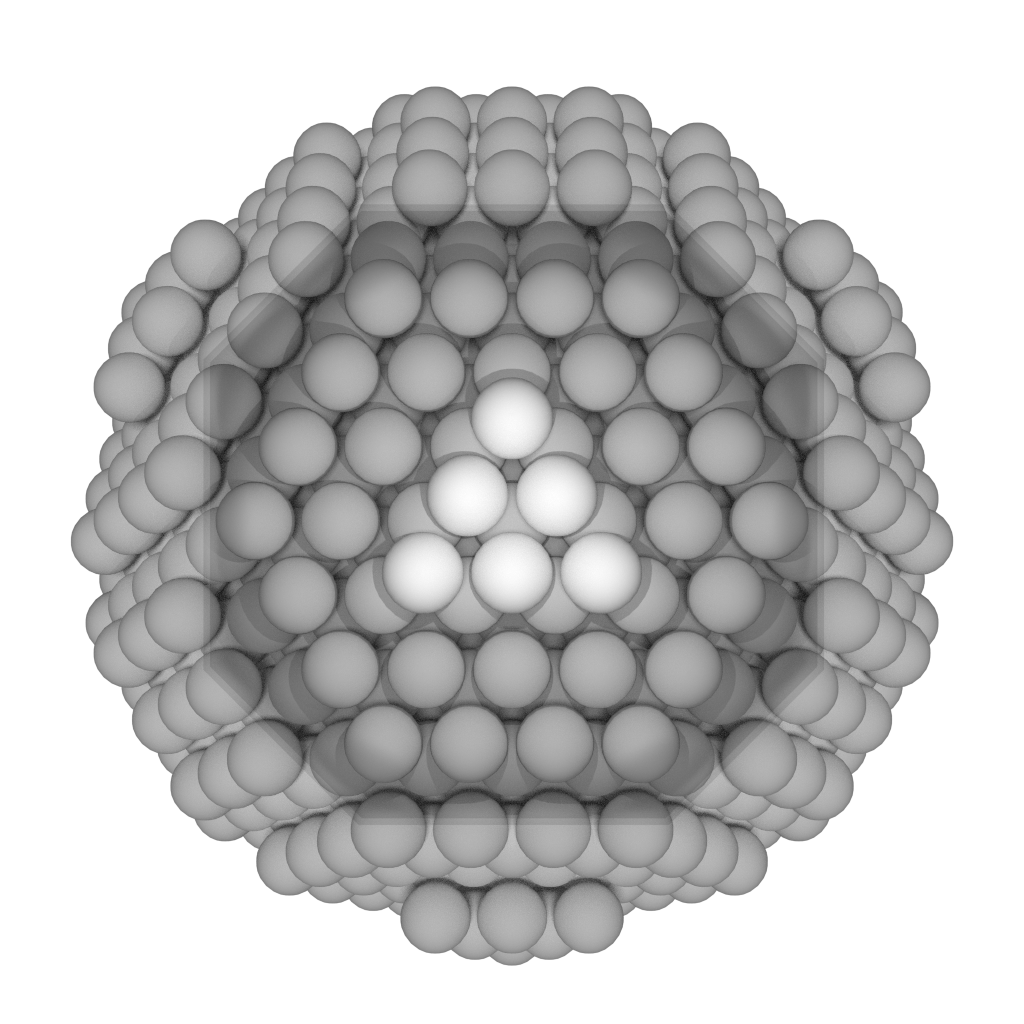
\includegraphics[width=0.3\textwidth]{./images/fcc-111-persp}} \quad
	\subfigure[(100)]{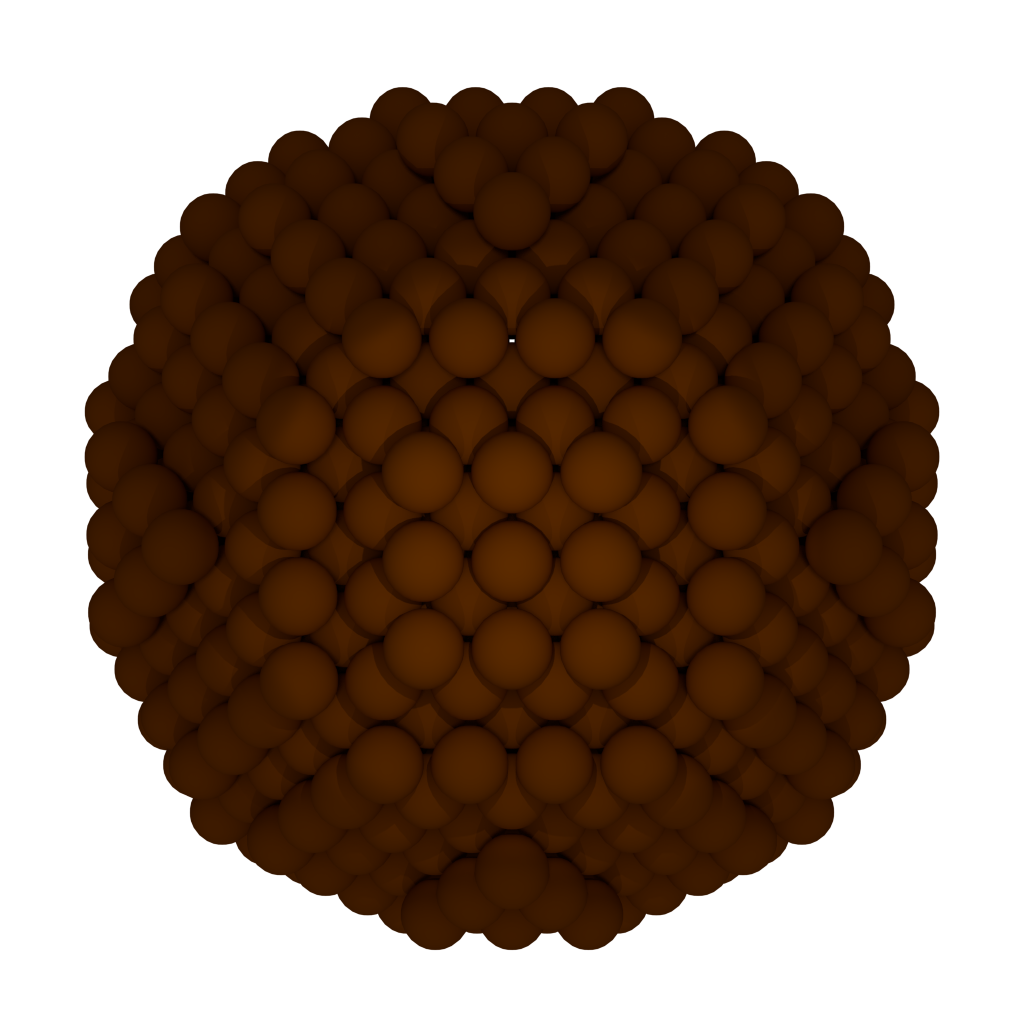
\includegraphics[width=0.3\textwidth]{./images/fcc-100-persp}}
%	\subfigure[(110)]{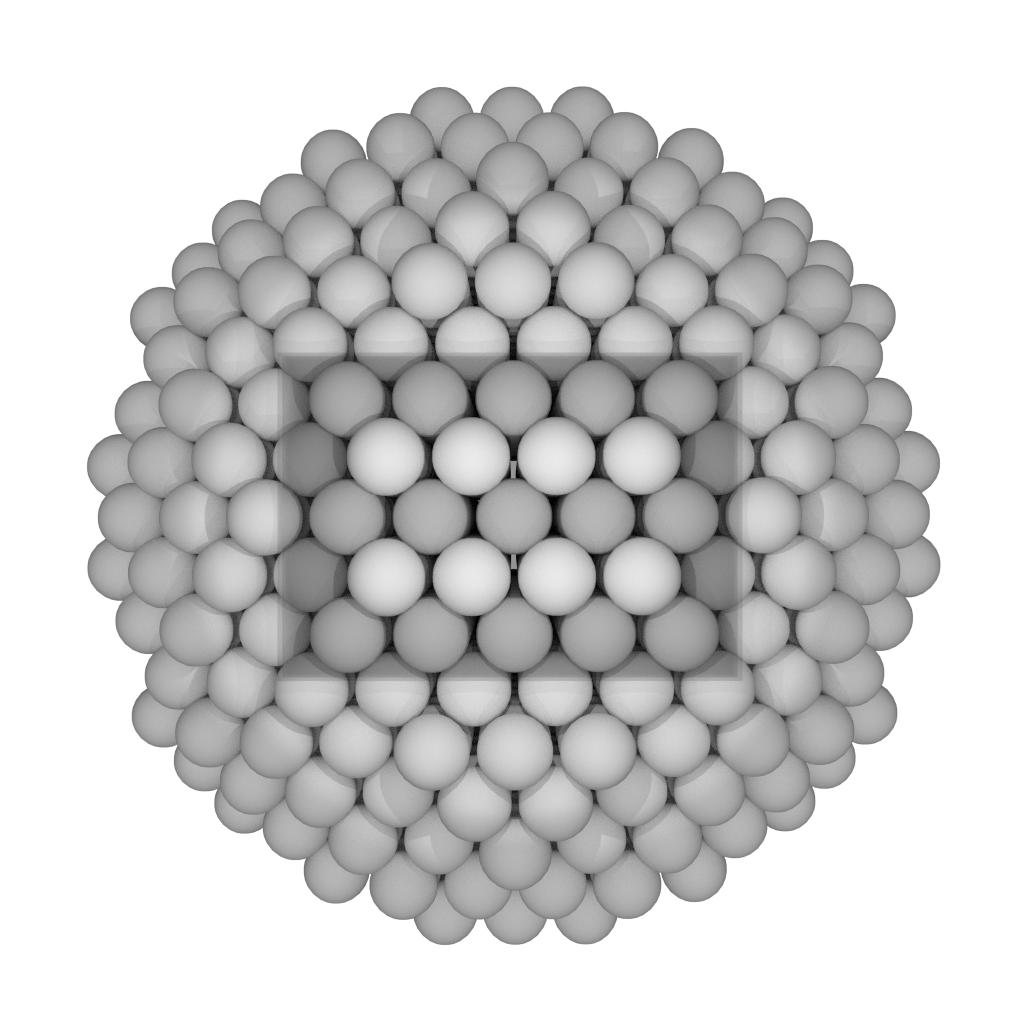
\includegraphics[width=0.3\textwidth]{./images/fcc-110-persp}}
	\caption{Identical crystalline balls in fcc lattice configuration. The surface termination is determined by the direction of the intersecting plane (parallel to the paper plane) relative to the lattice.}
	\label{fig:crystal-termination}
\end{figure}

The surface free energy increases from the (111) surface with increasing angle of the (hkl) planes of interest with $$\cos(\phi)=\frac{h+k+l}{\sqrt{3(h^2+k^2+l^2)}}$$ \cite{jian-min_calculation_2004}. Thus, the (111) surface is the one with lowest energy, followed by (110) and (100).


Dislocation lines and crystal orientation

Due to the fact, that dislocation lines move within the crystal in a well defined manner, one can determine the crystals orientation when the orientation of a dislocation is known.
For fcc crystals the orientation of dislocation lines occurs in the {111} plane in $<110>$ direction. Its Burgers vector is $\frac{a}{2}[110]$\cite{_dislocation-theory}. \underline{ADD INFO	FOR 100!!!}

 Dense packed rows in fcc(111) are the following directions: $<\bar 1 01>$, $<01\bar 1>$, $<1\bar 1 0>$. The diagonals are found in the $<\bar 1 \bar 1 2>$ and $<1\bar 2 1>$ directions. \underline{ADD INFO	FOR 100!!!}
 \subsection{Polycrystalline copper foils}
 As was mentioned before, clean, highly ordered surfaces are desirable to perform experiments on. Effort is done to clean the surfaces before every experiment to ensure a reproducible environment and interpretable results. This lead to a detailed understanding of the physics and chemistry behind a lot of systems. In case a systems order and functionality does not heavily depend on the substrates symmetry, single crystals loose most of their unique selling point. Instead of choosing a expensive bulk single crystal, thin copper foils can catch up in production environments. The mass produced foils still show some inconvenient properties. Although pure copper foils ($\geq \SI{99.999}{\percent}$) are available, their surface was never meant to be atomically flat. 
 A representation of a copper surface before electro polishing can be seen in figure \ref{fig:copper-foil-grains}. Here the layered structure of the (mechanically polished) foil is apparent and shows different sizes of grains and annealing twins at the surface. Small subgrains constitute the uppermost layers, while deeper lying layers consist of larger grains with grain boundaries becoming more and more diffuse with increasing distance to the surface.
 
To overcome these limitations, etching of the copper froil is performed as described in \autoref{sec:etching}